\chapter{Tecnologie}

\section{Stack tecnologico landing pages}
Il progetto di redesign delle landing pages si basa su uno stack moderno 
orientato a performance, SEO e developer experience. Le scelte tecnologiche 
sono state guidate dalla necessità di garantire caricamenti rapidi, 
indicizzazione ottimale sui motori di ricerca e scalabilità futura.

\subsection{Frontend}

Il framework principale è Next.js 15, che si basa su React 19 e TypeScript 
5.7. Queste tecnologie erano già in uso nel progetto precedente e sono 
state mantenute durante il redesign per coerenza con l'intero ecosistema 
tecnologico aziendale.

\paragraph{React 19}
React è la libreria JavaScript per costruire interfacce utente component-based, 
utilizzata in tutti i principali prodotti Datapizza (Jobs, Company, gestionale 
interno). Questa coerenza tecnologica garantisce riuso del codice, competenze 
consolidate del team e facilita l'inserimento di nuovi sviluppatori. L'approccio 
component-based permette di costruire interfacce modulari suddividendo 
l'interfaccia in componenti indipendenti e riutilizzabili, facilitando la 
manutenzione e la scalabilità del codice.

\paragraph{TypeScript 5.7}
A supporto di React è stato adottato TypeScript 5.7, un superset di 
JavaScript che aggiunge type safety statico, ormai standard per applicazioni 
moderne in contesti production. L'adozione di TypeScript riduce significativamente 
la probabilità di errori in produzione grazie al type checking in fase di 
sviluppo: errori comuni come accesso a proprietà inesistenti o passaggio di 
parametri errati vengono intercettati dal compilatore prima del deployment. 
In un contesto production come le landing pages, dove errori critici impattano 
direttamente le conversioni, TypeScript è fondamentale per garantire affidabilità.

TypeScript migliora significativamente il lavoro in team rendendo il codice più 
strutturato e auto-documentato. L'autocompletion intelligente negli IDE accelera 
lo sviluppo, mentre il supporto al refactoring permette modifiche strutturali 
sicure, riducendo il tempo di apprendimento per nuovi sviluppatori.

\paragraph{Next.js 15}
Next.js è un framework React ampiamente adottato per lo sviluppo di applicazioni 
production-ready, fornendo funzionalità avanzate di rendering e ottimizzazione. 
La scelta di Next.js rispetto a React standalone si basa su tre vantaggi 
fondamentali per il progetto.

Il rendering ibrido combina diverse strategie di generazione delle pagine: 
Server-Side Rendering (SSR) per generare HTML dinamico ad ogni richiesta, 
Static Site Generation (SSG) per pre-generare pagine statiche in fase di build, 
e Incremental Static Regeneration (ISR) che estende SSG permettendo 
l'aggiornamento incrementale di contenuti statici senza rigenerare l'intero 
sito. Questo approccio ottimizza sia i tempi di caricamento che la freschezza 
dei contenuti.

Il SEO nativo garantisce che i motori di ricerca ricevano HTML completo 
server-side, fondamentale per indicizzazione efficace e traffico organico. 
Il code splitting automatico suddivide il codice in bundle separati per 
ogni route, caricando solo lo stretto necessario per la pagina corrente 
e riducendo il tempo di primo caricamento.

Next.js supporta nativamente il routing internazionalizzato, esteso in questo 
progetto tramite la libreria next-intl per gestire i percorsi localizzati 
(/it/ e /en/). Il componente next/image ottimizza automaticamente le immagini: 
conversione in formato moderno (WebP/AVIF), caricamento differito quando 
l'immagine entra nel viewport (lazy loading), e generazione di varianti 
responsive per adattarsi alle dimensioni del dispositivo, riducendo il peso 
complessivo mantenendo qualità visiva.

\subsection{Styling e UI}

Per garantire coerenza visiva con l'identità aziendale, il sistema di styling 
si basa su Tailwind CSS integrato con la component library ShadCN UI.

Tailwind CSS è un framework CSS utility-first (approccio basato su classi 
utilitarie) che permette di costruire interfacce applicando classi predefinite 
direttamente nel markup HTML, eliminando la necessità di scrivere file CSS 
separati. A differenza dei framework tradizionali basati su componenti 
pre-stilizzati (come Bootstrap), Tailwind fornisce classi atomiche di basso 
livello che compongono lo stile finale. Durante la fase di build, solo le 
classi effettivamente utilizzate vengono compilate nel CSS finale, riducendo 
drasticamente le dimensioni del bundle e garantendo tempi di caricamento ridotti.

ShadCN UI completa l'infrastruttura di styling fornendo componenti accessibili 
basati sulle primitive Radix UI, con conformità nativa agli standard WCAG 2.1 
livello AA. A differenza delle librerie tradizionali, ShadCN UI genera i 
componenti direttamente nel progetto tramite command-line interface, garantendo 
pieno controllo sul codice senza dipendenze esterne rigide. L'integrazione con 
Tailwind permette di stilizzare i componenti con utility classes, combinando 
accessibilità e flessibilità di design.

\subsection{Librerie complementari}

Per animazioni e interattività avanzate, il progetto utilizza Framer Motion per 
animazioni fluide nelle sezioni principali (Hero sections) e Three.js con React 
Three Fiber per visualizzazioni 3D sulla landing AI Engineering. La gestione dei 
form si basa su React Hook Form per performance ottimali e Zod per validazione 
dello schema dati con supporto TypeScript integrato sui form di acquisizione lead.

Il tracking degli eventi utente è gestito tramite Mixpanel, piattaforma di 
product analytics che permette di tracciare interazioni personalizzate e 
costruire funnel di conversione differenziati per verticale. A differenza di 
strumenti generici come Google Analytics, Mixpanel offre granularità event-based: 
ogni interazione utente (click su call-to-action, scroll della pagina, apertura 
form) viene tracciata come evento discreto, permettendo analisi dettagliate del 
customer journey. L'SDK Mixpanel viene inizializzato lato client solo dopo 
consenso esplicito dell'utente tramite cookie banner, in conformità al GDPR 
mediante anonimizzazione degli indirizzi IP e gestione delle preferenze di 
privacy.

\subsection{Backend per dati dinamici}

Alcune funzionalità delle landing pages richiedono elaborazioni lato server 
che il frontend non può gestire autonomamente, come la validazione sicura dei 
form, l'integrazione con servizi esterni e l'accesso al database aziendale.

Il backend è condiviso tra tutti i prodotti Datapizza: oltre alle landing pages, 
serve le applicazioni Jobs (lato candidati), Company (lato aziende) e il CRM 
interno. Questa architettura unificata consente una manutenzione centralizzata 
e garantisce consistenza dei dati tra piattaforme.

\paragraph{Django e Python}
Il backend si basa su Django, framework web scritto in Python. Python è un 
linguaggio di programmazione ad alto livello, apprezzato per la sua semplicità 
sintattica e il vasto ecosistema di librerie, particolarmente ricco nell'ambito 
data science e intelligenza artificiale. Django fornisce un'architettura robusta 
per costruire API REST in modo rapido e sicuro, con strumenti integrati per 
autenticazione, gestione database e validazione dati.

\paragraph{PostgreSQL}
Il database utilizzato è PostgreSQL, sistema di gestione database relazionale 
open-source. PostgreSQL organizza i dati in tabelle strutturate collegate tra 
loro tramite relazioni, garantendo integrità referenziale e consistenza. Nel 
contesto del progetto, PostgreSQL gestisce le opportunità lavorative visualizzate 
sulla Jobs Platform, i dati degli utenti registrati e le informazioni aziendali.

\paragraph{Funzionalità principali}
Il backend gestisce diverse integrazioni critiche per il funzionamento delle 
landing pages. I form di contatto passano attraverso validazione lato server 
per prevenire input malevoli e garantire che solo dati validi raggiungano il 
database. L'integrazione con Customer.io, piattaforma di email automation, 
gestisce le iscrizioni alla newsletter "Commit" e l'invio di comunicazioni 
personalizzate agli oltre 500.000 iscritti della community. Il sistema fornisce 
inoltre API per il recupero in tempo reale delle opportunità lavorative 
visualizzate sulla Jobs Platform.

Deployato su infrastruttura cloud AWS, lo stack backend completo si basa su 
Django 4.x, PostgreSQL 15 e Python 3.9, per garantire scalabilità e disponibilità. 
L'infrastruttura di deployment su AWS è dettagliata nel Capitolo 7, mentre 
la Figura~\ref{fig:stack-landing} illustra l'architettura applicativa 
complessiva delle landing pages.

\begin{figure}[h!]
    \centering
    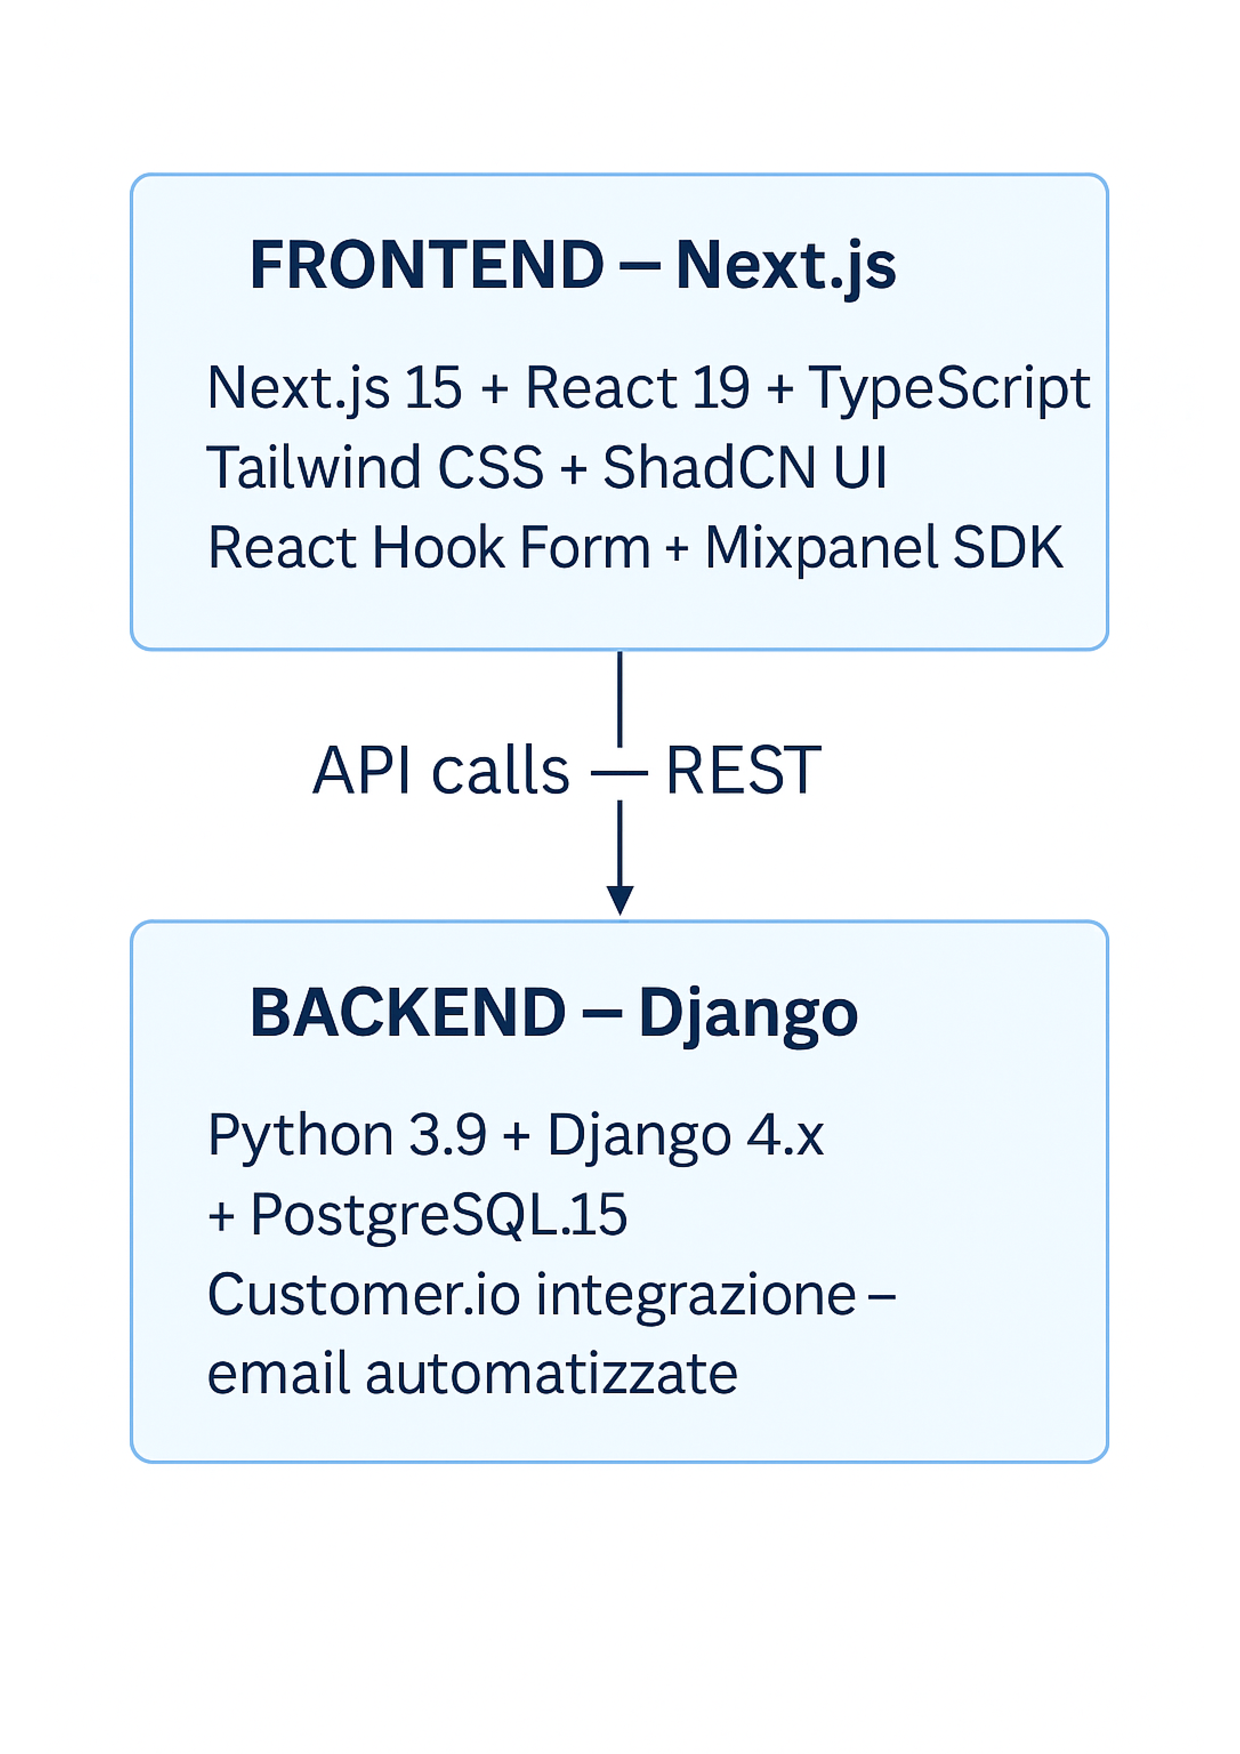
\includegraphics[width=0.52\textwidth]{chapters/figures/stack2.pdf}
    \caption{Architettura applicativa delle landing pages che mostra 
    l'interazione tra frontend e backend 
 tramite API REST.}
    \label{fig:stack-landing}
\end{figure}

\clearpage

\section{Stack tecnologico aziendale}

L'ecosistema Datapizza (Jobs, Company, gestionale, landing pages) condivide 
uno stack unificato per garantire coerenza tecnologica e riutilizzo di competenze 
tra prodotti. La Tabella~\ref{tab:stack-aziendale} fornisce una panoramica 
completa delle tecnologie adottate a livello aziendale.

\begin{table}[h]
\centering
\caption{Stack tecnologico aziendale}
\label{tab:stack-aziendale}
\begin{tabular}{|l|l|p{6.5cm}|}
\hline
\textbf{Layer} & \textbf{Tecnologie} & \textbf{Note} \\
\hline
Frontend & React 19, TypeScript 5.7 & Base comune tutti i prodotti \\
\hline
Frontend & React Query & State management server-side \\
\hline
Frontend & TanStack Router & Routing type-safe (CRM) \\
\hline
Backend & Django 4.x, PostgreSQL 15 & Stack verticale Python \\
\hline
Infrastructure & AWS (eu-south-1) & Cloud provider \\
\hline
Infrastructure & Docker, AWS ECR & Containerizzazione \\
\hline
Infrastructure & S3, CloudFront & Storage e distribuzione globale \\
\hline
Infrastructure & Lambda & Integrazioni AI serverless \\
\hline
Tools & Mixpanel & Analytics GDPR-compliant \\
\hline
Tools & Customer.io & Email automation (500k+ iscritti) \\
\hline
\end{tabular}
\end{table}

\section{Development tools e workflow}

Il team utilizza una suite integrata di strumenti per garantire efficienza, 
qualità del codice e collaborazione efficace. La Tabella~\ref{tab:dev-tools} 
riassume le principali tecnologie adottate.

\clearpage
\begin{table}[h]
\centering
\caption{Strumenti di sviluppo e workflow}
\label{tab:dev-tools}
\begin{tabular}{|l|l|p{6cm}|}
\hline
\textbf{Categoria} & \textbf{Tecnologia} & \textbf{Utilizzo} \\
\hline
IDE & VS Code + Cursor AI & Editor principale con AI assistance \\
\hline
Version Control & GitLab self-hosted & Repository privato, Merge Request \\
\hline
Project Management & Jira & Task tracking, sprint planning \\
\hline
Deployment & Docker + AWS ECR & Containerizzazione e registry \\
\hline
Communication & Discord, Google Meet & Daily standup, sync team \\
\hline
Documentation & Notion & Knowledge base, onboarding \\
\hline
\end{tabular}
\end{table}

Il workflow di sviluppo segue approccio Agile con sprint bisettimanali. Il 
codice viene sviluppato su branch Git dedicati per ogni nuova funzionalità 
(feature branches), e ogni modifica richiede Merge Request su GitLab con 
revisione del codice (code review) obbligatoria da parte di almeno un 
collega prima dell'integrazione nel branch principale. Jira traccia le user 
stories con stima della complessità in story points, mentre grafici di 
avanzamento (burndown charts) monitorano il progresso di ogni sprint. La 
documentazione tecnica è centralizzata su Notion per garantire accessibilità 
rapida a tutto il team.